\documentclass[12pt]{article}
\usepackage{amsmath}
\usepackage{graphicx}
\usepackage{hyperref}
\usepackage{listings}
\usepackage{color}
\usepackage{pythonhighlight}

\title{Operating System Course Report - First Half of the Semester}
\author{B class}
\date{\today}

\begin{document}

\maketitle
\newpage

\tableofcontents
\newpage

\section{Introduction}
This report summarizes the topics covered during the first half of the Operating System course. It includes theoretical concepts, practical implementations, and assignments. The course focuses on the fundamentals of operating systems, including system architecture, process management, CPU scheduling, and deadlock handling.

\section{Course Overview}
\subsection{Objectives}
The main objectives of this course are:
\begin{itemize}
    \item To understand the basic components and architecture of a computer system.
    \item To learn process management, scheduling, and inter-process communication.
    \item To explore file systems, input/output management, and virtualization.
    \item To study the prevention and handling of deadlocks in operating systems.
\end{itemize}

\subsection{Course Structure}
The course is divided into two halves. This report focuses on the first half, which covers:
\begin{itemize}
    \item Basic Concepts and Components of Computer Systems
    \item System Performance and Metrics
    \item System Architecture of Computer Systems
    \item Process Description and Control
    \item Scheduling Algorithms
    \item Process Creation and Termination
    \item Introduction to Threads
    \item File Systems
    \item Input and Output Management
    \item Deadlock Introduction and Prevention
    \item User Interface Management
    \item Virtualization in Operating Systems
\end{itemize}

\section{Topics Covered}

\subsection{Basic Concepts and Components of Computer Systems}
This section explains the fundamental components that make up a computer system, including the CPU, memory, storage, and input/output devices.

\subsection{System Performance and Metrics}
This section introduces various system performance metrics used to measure the efficiency of a computer system, including throughput, response time, and utilization.

\subsection{System Architecture of Computer Systems}
Describes the architecture of modern computer systems, focusing on the interaction between hardware and the operating system.

\subsection{Process Description and Control}
Processes are a central concept in operating systems. This section covers:
\begin{itemize}
    \item Process states and state transitions
    \item Process control block (PCB)
    \item Context switching
\end{itemize}

\subsection{Scheduling Algorithms}
This section covers:
\begin{itemize}
    \item First-Come, First-Served (FCFS)
    \item Shortest Job Next (SJN)
    \item Round Robin (RR)
\end{itemize}
It explains how these algorithms are used to allocate CPU time to processes.

\subsection{Process Creation and Termination}
Details how processes are created and terminated by the operating system, including:
\begin{itemize}
    \item Process spawning
    \item Process termination conditions
\end{itemize}

\subsection{Introduction to Threads}
This section introduces the concept of threads and their relation to processes, covering:
\begin{itemize}
    \item Single-threaded vs. multi-threaded processes
    \item Benefits of multithreading
\end{itemize}

\begin{figure}[h]
    \centering
    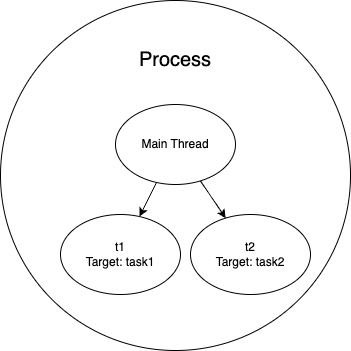
\includegraphics[width=0.5\textwidth]{/Users/khawaritzmi/Unhas/os_report_mid2024/b_class/asset/example.png}  % Sesuaikan nama file dan ukurannya
    \caption{Ini adalah gambar contoh dari multithreading.}
    \label{fig:contoh_gambar}
\end{figure}

Seperti yang terlihat pada Gambar \ref{fig:contoh_gambar}, inilah cara menambahkan gambar dengan keterangan.

\subsection{File Systems}
File systems provide a way for the operating system to store, retrieve, and manage data. This section explains:
\begin{itemize}
    \item File system structure
    \item File access methods
    \item Directory management
\end{itemize}

\subsection{Input and Output Management}
Input and output management is key for handling the interaction between the system and external devices. This section includes:
\begin{itemize}
    \item Device drivers
    \item I/O scheduling
\end{itemize}

\subsection{Deadlock Introduction and Prevention}
Explores the concept of deadlocks and methods for preventing them:
\begin{itemize}
    \item Deadlock conditions
    \textbf{Deadlock Avoidance} 

Deadlock avoidance adalah teknik yang digunakan untuk mencegah sistem komputer masuk ke dalam situasi deadlock, yaitu ketika beberapa proses tidak dapat melanjutkan karena saling menunggu sumber daya yang dipegang oleh proses lain. Prinsip utama dari deadlock avoidance adalah menjaga sistem agar selalu berada dalam \textit{safe state}, di mana deadlock tidak mungkin terjadi.
\begin{itemize}
\item \textbf{Ide Dasar Deadlock Avoidance}: Deadlock avoidance bertujuan untuk memastikan bahwa sistem tidak pernah berada dalam \textit{unsafe state}, di mana kemungkinan deadlock bisa terjadi. Hal ini dilakukan dengan menganalisis dan memperkirakan permintaan sumber daya yang mungkin akan diminta oleh setiap proses sebelum mereka benar-benar diberikan.
\item \textbf{Kebutuhan Informasi tentang Permintaan Sumber Daya}: Teknik ini membutuhkan informasi sebelumnya tentang bagaimana proses-proses yang berbeda akan meminta sumber daya di masa depan. Dengan mengetahui berapa banyak dan kapan proses akan meminta sumber daya, sistem dapat memutuskan apakah permintaan tersebut aman untuk dipenuhi atau tidak.
\item \textbf{Safe State (State Aman)}: \textit{Safe state} adalah kondisi di mana sistem dapat memberikan semua permintaan sumber daya dari proses-prosesnya tanpa menyebabkan deadlock. Dalam state ini, ada urutan eksekusi proses yang memungkinkan semua proses menyelesaikan tugasnya.
\item \textbf{Unsafe State (State Tidak Aman)}: \textit{Unsafe state} terjadi ketika sistem berada dalam kondisi di mana ada kemungkinan deadlock, meskipun tidak terjadi secara langsung. Di dalam \textit{unsafe state}, jika proses-proses meminta sumber daya tertentu yang tidak tersedia, deadlock dapat terjadi.

\end{itemize}
\textbf{Deadlock Detection} 
Deadlock detection adalah strategi yang memungkinkan deadlock terjadi dalam sistem terlebih dahulu, kemudian mendeteksinya, dan melakukan tindakan \textit{recovery} untuk mengembalikan sistem ke keadaan normal. Deadlock detection berfokus pada pemantauan sistem dan mengambil langkah korektif ketika deadlock terdeteksi.
\begin{itemize}
\item \textbf{Ide Dasar Deadlock Detection}: Deadlock detection tidak mencegah deadlock dari awal, tetapi mengizinkan deadlock untuk terjadi dan kemudian mendeteksi keberadaannya. Setelah deadlock terdeteksi, sistem melakukan langkah \textit{recovery}.
\item \textbf{Membatalkan Semua Proses yang Terlibat dalam Deadlock}: Salah satu solusi yang ekstrem adalah membatalkan atau menghentikan semua proses yang terlibat dalam deadlock. Meskipun ini akan secara efektif menyelesaikan deadlock, pendekatan ini sering kali tidak efisien karena dapat menyebabkan hilangnya banyak pekerjaan yang sudah dilakukan oleh proses tersebut.
\item \textbf{Membatalkan Satu Proses pada Satu Waktu hingga Deadlock Teratasi}: Alternatif yang lebih efisien adalah membatalkan satu proses pada satu waktu. Proses yang dibatalkan dipilih berdasarkan kriteria tertentu, seperti proses yang memiliki prioritas lebih rendah atau proses yang sudah menggunakan lebih sedikit sumber daya. Proses ini diulang hingga siklus deadlock dapat dihilangkan.
\item \textbf{Preemption (Pengambilalihan Sumber Daya)}: Teknik lain untuk \textit{recovery} adalah dengan \textit{preemption}, yaitu mengambil sumber daya dari satu atau lebih proses yang sedang menjalankan tugasnya. Sumber daya yang telah diambil bisa diberikan ke proses lain yang memerlukan untuk melanjutkan eksekusi dan memecah siklus deadlock.
\item \textbf{Checkpoint dan Rollback}: Sistem dapat melakukan \textit{checkpoint}, yaitu menyimpan status proses di titik tertentu. Jika deadlock terdeteksi, sistem bisa melakukan \textit{rollback}, yaitu mengembalikan proses ke \textit{checkpoint} terakhir, lalu memulai ulang proses. Proses yang memiliki prioritas lebih rendah atau yang menyebabkan deadlock bisa dihentikan untuk menyelesaikan masalah.
\end{itemize}
\paragraph{Kesimpulan tentang Deadlock}
\textbf{Deadlock} adalah kondisi dalam sistem komputer di mana satu atau lebih proses tidak dapat melanjutkan eksekusi karena saling menunggu sumber daya yang sedang dipegang oleh proses lain. Dalam keadaan deadlock, proses-proses ini tidak akan pernah selesai kecuali jika dilakukan tindakan \textit{recovery} untuk memecah siklus deadlock tersebut.
{Empat Kondisi Penting untuk Terjadinya Deadlock}
\begin{itemize}
\item \textit{Mutual Exclusion} (Saling Mengunci): Sumber daya tidak dapat digunakan oleh lebih dari satu proses pada saat yang bersamaan.
\item \textit{Hold and Wait} (Menahan dan Menunggu): Proses yang telah memiliki beberapa sumber daya menahan sumber daya tersebut sambil menunggu sumber daya lain yang sedang digunakan oleh proses lain.
\item \textit{No Preemption} (Tidak Ada Pengambilalihan): Sumber daya yang telah dialokasikan ke suatu proses tidak dapat diambil alih secara paksa dari proses tersebut, hanya bisa dilepaskan secara sukarela oleh proses yang sedang menggunakannya.
\item \textit{Circular Wait} (Tunggu Melingkar): Terdapat rangkaian proses yang menunggu secara melingkar, di mana setiap proses dalam siklus menunggu sumber daya yang dimiliki oleh proses berikutnya dalam siklus.

\end{itemize}
Ada empat strategi utama untuk menangani deadlock:
\begin{itemize}
\item \textit{Prevention} (Pencegahan): Mencegah terjadinya salah satu atau lebih dari empat kondisi deadlock. Misalnya, dengan memastikan tidak ada \textit{hold and wait} atau memperbolehkan \textit{preemption}.
\item \textit{Avoidance} (Penghindaran): Sistem memantau statusnya secara dinamis dan hanya mengalokasikan sumber daya jika tidak menyebabkan \textit{unsafe state} yang berpotensi menyebabkan deadlock. Contoh metode penghindaran adalah \textit{Banker’s Algorithm}.
\item \textit{Detection} (Deteksi): Deadlock diizinkan untuk terjadi, tetapi sistem memiliki mekanisme untuk mendeteksinya setelah itu. Ketika deadlock terdeteksi, sistem kemudian mengambil tindakan untuk \textit{recovery}.
\item \textit{Recovery} (Pemulihan): Setelah deadlock terdeteksi, sistem dapat melakukan berbagai tindakan untuk memulihkan keadaan, seperti membatalkan proses, mengambil sumber daya dari proses, atau menggunakan \textit{checkpoint} dan \textit{rollback}.
\end{itemize}
    \item Deadlock prevention techniques
\end{itemize}

\subsection{User Interface Management}
This section discusses the role of the operating system in managing the user interface. Topics covered include:
\begin{itemize}
    \item Graphical User Interface (GUI)
    \item Command-Line Interface (CLI)
    \item Interaction between the user and the operating system
\end{itemize}

\subsection{Virtualization in Operating Systems}
Virtualization allows multiple operating systems to run concurrently on a single physical machine. This section explores:
\begin{itemize}
    \item Concept of virtualization
    \item Hypervisors and their types
    \item Benefits of virtualization in modern computing
\end{itemize}

\section{Assignments and Practical Work}
\subsection{Assignment 1: Process Scheduling}
Students were tasked with implementing various process scheduling algorithms (e.g., FCFS, SJN, and RR) and comparing their performance under different conditions.
\subsubsection{Group 1}
\begin{python}
    class Process:
    def __init__(self, pid, arrival_time, burst_time):
        self.pid = pid
        self.arrival_time = arrival_time
        self.burst_time = burst_time
        self.completion_time = 0
        self.turnaround_time = 0
        self.waiting_time = 0
\end{python}

\begin{table}[htbp] % Optional: For floating position
    \centering
    \begin{tabular}{|c|c|c|} % Defines number of columns and alignment (c = center, l = left, r = right). '|' creates vertical lines.
    \hline
    Header 1 & Header 2 & Header 3 \\ % Column headers
    \hline
    Row 1, Column 1 & Row 1, Column 2 & Row 1, Column 3 \\ % First row of data
    \hline
    Row 2, Column 1 & Row 2, Column 2 & Row 2, Column 3 \\ % Second row of data
    \hline
    \end{tabular}
    \caption{Your table caption} % Optional: For adding a caption
    \label{tab:your_label} % Optional: For cross-referencing the table
\end{table}

\subsection{Assignment 2: Deadlock Handling}
In this assignment, students were asked to simulate different deadlock scenarios and explore various prevention methods.

\subsection{Assignment 3: Multithreading and Amdahl's Law}
This assignment involved designing a multithreading scenario to solve a computationally intensive problem. Students then applied **Amdahl's Law** to calculate the theoretical speedup of the program as the number of threads increased.

\subsection{Assignment 4: Simple Command-Line Interface (CLI) for User Interface Management}
Students were tasked with creating a simple **CLI** for user interface management. The CLI should support basic commands such as file manipulation (creating, listing, and deleting files), process management, and system status reporting.

\subsection{Assignment 5: File System Access}
In this assignment, students implemented file system access routines, including:
\begin{itemize}
     \item File creation and deletion
    \item Reading from and writing to files
    \item Navigating directories and managing file permissions
\end{itemize}
\subsubsection{Group 10}



\textbf{No 1}


    Gunakan Python dan modul bawaan seperti ⁠ os ⁠ dan ⁠ shutil ⁠ untuk mengimplementasikan operasi ini. Tulis kode yang akan melakukan hal berikut:
\begin{enumerate}
    \item Membuat sebuah direktori baru bernama \texttt{test\_dir}.
    \item Membuat file baru di dalam direktori tersebut bernama \texttt{example.txt} dan menulis teks ke file itu.
    \item Membaca konten dari file \texttt{example.txt}.
    \item Menghapus file \texttt{example.txt}.
    \item Mengatur izin file dalam direktori \texttt{test\_dir} untuk membuat file hanya dapat dibaca.
\end{enumerate}
\textit{JAWABAN :}
\begin{python}
import os
import shutil

def create_directory(directory_name):
    if not os.path.exists(directory_name):
        os.makedirs(directory_name)
        print(f"Directory '{directory_name}' created.")
    else:
        print(f"Directory '{directory_name}' already exists.")

def create_file(file_path, content):
    with open(file_path, 'w') as file:
        file.write(content)
        print(f"File '{file_path}' created and written.")

def read_file(file_path):
    if os.path.exists(file_path):
        with open(file_path, 'r') as file:
            content = file.read()
            print(f"Reading from '{file_path}':\n{content}")
    else:
        print(f"File '{file_path}' does not exist.")

def delete_file(file_path):
    if os.path.exists(file_path):
        os.remove(file_path)
        print(f"File '{file_path}' deleted.")
    else:
        print(f"File '{file_path}' does not exist.")

def change_permissions(directory_path):
    if os.path.exists(directory_path):
        # Set read-only permission to the directory and its contents
        os.chmod(directory_path, 0o444)
        print(f"Permissions for directory '{directory_path}' set to read-only.")
    else:
        print(f"Directory '{directory_path}' does not exist.")

# Assignment steps implementation
dir_name = 'test_dir'
file_name = 'example.txt'
file_path = os.path.join(dir_name, file_name)

# Step 1: Create a directory
create_directory(dir_name)

# Step 2: Create a file and write to it
create_file(file_path, "This is a test file for file system access assignment.")

# Step 3: Read the file
read_file(file_path)

# Step 4: Delete the file
delete_file(file_path)

# Step 5: Change permissions of the directory to read-only
change_permissions(dir_name)
\end{python}

\textit{PENJELASAN :}
\begin{enumerate}
    \item Fungsi \textit{create\_directory} digunakan untuk membuat direktori baru dengan nama yang ditentukan jika direktori tersebut belum ada.
    \item Fungsi \textit{create\_file} membuka file dalam mode tulis dan menulis teks yang diberikan ke file. Jika file belum ada, maka akan dibuat.
    \item Fungsi \textit{read\_file} membaca dan menampilkan isi file jika file ada. Ini menggunakan metode pembacaan standar dalam Python.
    \item Fungsi \textit{delete\_file} digunakan untuk menghapus file jika file tersebut ada di sistem.
    \item Fungsi \textit{change\_permissions} mengatur izin file atau direktori menjadi hanya-baca (\textit{read-only}) menggunakan ⁠ os.chmod() ⁠.

\end{enumerate}
    Program di atas menciptakan direktori baru bernama ⁠ test\_dir ⁠, membuat file ⁠ example.txt ⁠ di dalamnya, menulis teks ke dalam file, membaca isi file, menghapus file, dan mengatur izin direktori agar menjadi hanya-baca.
\end{enumerate}

\section{Conclusion}
The first half of the course introduced core operating system concepts, including process management, scheduling, multithreading, and file system access. These topics provided a foundation for more advanced topics to be covered in the second half of the course.

\end{document}
